\documentclass{article}
\usepackage[utf8]{inputenc}
\usepackage[T1]{fontenc}

% Set page geometry
\usepackage[margin=2.5cm,headsep=0.5cm]{geometry}

% AMS and mathtools
\usepackage{amsmath,amsthm,amssymb,marvosym,mathrsfs,amsfonts,amscd,mathtools}

% Hyperlinks and URLs
\usepackage{url}
\usepackage{hyperref}
\hypersetup{
    colorlinks,
    citecolor=black,
    filecolor=black,
    linkcolor=black,
    urlcolor=black
}

% Colors
\usepackage{xcolor}

% Bold math
\usepackage{bm}

% Bra Ket (Dirac) Notation
\usepackage{braket}

% Slashed characters (e.g. in Dirac equation)
\usepackage{slashed}

% Clean SI Units
\usepackage{siunitx}

% Enumerate thingies
\usepackage{enumitem}

% Cancel things out in equations
\usepackage[makeroom]{cancel}

% Graphics and figures
\usepackage{graphicx}
\usepackage{wrapfig}
\usepackage{float}

% Caption figures and tables
\usepackage{caption,subcaption}

% Generate symbols
\usepackage{textcomp} % Avoid output errors
\usepackage{gensymb}

% Make multiple rows in a table
\usepackage{multirow}

% Booktabs tables
\usepackage{booktabs}

% Useful frames
\usepackage{mdframed}

% Comment-out large sections
\usepackage{comment}

% No auto-indent
\setlength{\parindent}{0pt}

% Asymptote - 3D vector graphics
\usepackage{asymptote}

% Tikz Package Stuff
\usepackage{pgf,tikz,pgfplots}
\usepackage{tikz-3dplot}
% Use various tikz libraries
\usetikzlibrary{decorations.pathmorphing, decorations.markings, decorations.pathreplacing, patterns} % Decorate paths!
\usetikzlibrary{calc}
\usetikzlibrary{scopes}
\usetikzlibrary{angles, quotes}
\usetikzlibrary{svg.path}
\usetikzlibrary{arrows, arrows.meta}
\usetikzlibrary{fadings}
% pgfplots package settings
\pgfplotsset{compat=1.15}
% \pgfplotsset{width=10cm,compat=1.9} % From overleaf I think

% Awesome circled numbers
\newcommand*\circled[4]{\tikz[baseline=(char.base)]{\node[shape=circle, fill=#2, draw=#3, text=#4, inner sep=2pt] (char) {#1};}}

% Control size of text
\usepackage{relsize}

% Extend conditional commands
\usepackage{xifthen}

% Scale math by size
\newcommand*{\Scale}[2][4]{\scalebox{#1}{\ensuremath{#2}}}

% Big integrals
\usepackage{bigints}

% Generate blind text
\usepackage{blindtext}

% Useful symbols
\usepackage{marvosym}


%%%% THEOREMS %%%%
\newenvironment{theorem}[1][\hspace{-0.36em}]
{
    \begin{mdframed}[backgroundcolor=black!4, align=center, userdefinedwidth=40em, topline=false, bottomline = false, leftline = false, rightline = false, frametitle = {#1 Theorem}]
}
{
    \end{mdframed}
}

%%%% LEMMAS %%%%
\newenvironment{lemma}[1][\hspace{-0.36em}]
{
    \begin{mdframed}[backgroundcolor=black!4, align=center, userdefinedwidth=40em, topline=false, bottomline = false, leftline = false, rightline = false, frametitle = {#1 Lemma}]
}
{
    \end{mdframed}
}

%%%% COROLLARY %%%%
\newenvironment{corollary}[1][\hspace{-0.36em}]
{
    \begin{mdframed}[backgroundcolor=black!4, align=center, userdefinedwidth=40em, topline=false, bottomline = false, leftline = false, rightline = false, frametitle = {#1 Corollary}]
}
{
    \end{mdframed}
}

%%%% DEFINITIONS %%%%
\newenvironment{definition}[1][\hspace{-0.36em}]
{
    \begin{mdframed}[backgroundcolor=black!4, align=center, userdefinedwidth=40em, topline=false, bottomline = false, leftline = false, rightline = false, frametitle = {#1 Definition}]
}
{
    \end{mdframed}
}

%%%% PROPOSITION %%%%
\newenvironment{proposition}
{
    \begin{mdframed}[backgroundcolor=black!4, align=center, userdefinedwidth=40em, topline=false, bottomline = false, leftline = false, rightline = false, frametitle = {Proposition}]
}
{
    \end{mdframed}
}

% Change end-of-proof symbol
\renewcommand\qedsymbol{$\blacksquare$}


%%%% BLACKBOARD BOLD %%%%
\newcommand{\bbN}{\mathbb{N}} % Natural numbers
\newcommand{\bbZ}{\mathbb{Z}} % Zahlen
\newcommand{\bbQ}{\mathbb{Q}} % Rational numbers
\newcommand{\bbR}{\mathbb{R}} % Real numbers
\newcommand{\bbC}{\mathbb{C}} % Complex numbers
\DeclareSymbolFont{bbold}{U}{bbold}{m}{n} % Identity matrix
\DeclareSymbolFontAlphabet{\mathbbold}{bbold} % Identity matrix
\newcommand{\identitymatrix}{\mathbbold{1}} % Identity matrix


%%%% CODE LISTING %%%%
\usepackage{listings}
\definecolor{greencomments}{HTML}{00BA00}
\definecolor{graynumbers}{HTML}{4F4F4F}
\definecolor{purplestrings}{HTML}{AD00AA}
\definecolor{backgroundcolor}{HTML}{E8E8E8}
\lstdefinestyle{nkostin}{
    backgroundcolor=\color{backgroundcolor},
    commentstyle=\color{greencomments},
    keywordstyle=\color{blue},
    numberstyle=\tiny\color{graynumbers},
    stringstyle=\color{purplestrings},
    basicstyle=\footnotesize,
    breakatwhitespace=false,
    breaklines=true,
    captionpos=b,
    keepspaces=true,
    numbers=left,
    numbersep=5pt,
    showspaces=false,
    showstringspaces=false,
    showtabs=false,
    tabsize=2
}
\lstset{style=nkostin}

%%%% UNIT BASIS VECTORS %%%%
\newcommand{\ihat}{\bm{\hat{\imath}}} % Cartesian i hat (x-direction)
\newcommand{\jhat}{\bm{\hat{\jmath}}} % Cartesian j hat (y-direction)
\newcommand{\khat}{\bm{\hat{k}}} % Cartesian k hat (z-direction)
\newcommand{\rhat}{\bm{\hat{r}}} % Spherical r hat
\newcommand{\phihat}{\bm{\hat{\phi}}} % Spherical phi hat
\newcommand{\thetahat}{\bm{\hat{\theta}}} % Spherical theta hat
\newcommand{\nhat}{\bm{\hat{n}}} % Unit normal vector
\newcommand{\rhohat}{\bm{\hat{\rho}}} % Cylindrical rho hat
\newcommand{\zhat}{\bm{\hat{z}}} % Cylindrical z hat


%%%% COLORS: DEFINITIONS AND COMMANDS %%%%

\definecolor{nkostincolor}{HTML}{040080} % my favorite color
\newcommand{\nkostincolor}{\color{nkostincolor}}

%%%% RED %%%%
\definecolor{lightsalmon}{HTML}{FFA07A}
\definecolor{salmon}{HTML}{FA8072}
\definecolor{darksalmon}{HTML}{E9967A}
\definecolor{lightcoral}{HTML}{F08080}
\definecolor{indianred}{HTML}{CD5C5C}
\definecolor{crimson}{HTML}{DC143C}
\definecolor{firebrick}{HTML}{B22222}
\definecolor{red}{HTML}{FF0000}
\definecolor{darkred}{HTML}{8B0000}

%%%% ORANGE %%%%
\definecolor{coral}{HTML}{FF7F50}
\definecolor{tomato}{HTML}{FF6347}
\definecolor{orangered}{HTML}{FF4500}
\definecolor{gold}{HTML}{FFD700}
\definecolor{orange}{HTML}{FFA500}
\definecolor{darkorange}{HTML}{FF8C00}

%%%% YELLOW %%%%
\definecolor{lightyellow}{HTML}{FFFFE0}
\definecolor{lemonchiffon}{HTML}{FFFACD}
\definecolor{lightgoldenrodyellow}{HTML}{FAFAD2}
\definecolor{papayawhip}{HTML}{FFEFD5}
\definecolor{moccasin}{HTML}{FFE4B5}
\definecolor{peachpuff}{HTML}{FFDAB9}
\definecolor{palegoldenrod}{HTML}{EEE8AA}
\definecolor{khaki}{HTML}{F0E68C}
\definecolor{darkkhaki}{HTML}{BDB76B}
\definecolor{yellow}{HTML}{FFFF00}

%%%% GREEN %%%%
\definecolor{lawngreen}{HTML}{7CFC00}
\definecolor{chartreuse}{HTML}{7FFF00}
\definecolor{limegreen}{HTML}{32CD32}
\definecolor{lime}{HTML}{00FF00}
\definecolor{forestgreen}{HTML}{228B22}
\definecolor{green}{HTML}{008000}
\definecolor{darkgreen}{HTML}{006400}
\definecolor{greenyellow}{HTML}{ADFF2F}
\definecolor{yellowgreen}{HTML}{9ACD32}
\definecolor{springgreen}{HTML}{00FF7F}
\definecolor{mediumspringgreen}{HTML}{00FA9A}
\definecolor{lightgreen}{HTML}{90EE90}
\definecolor{palegreen}{HTML}{98FB98}
\definecolor{darkseagreen}{HTML}{8FBC8F}
\definecolor{mediumseagreen}{HTML}{3CB371}
\definecolor{seagreen}{HTML}{2E8B57}
\definecolor{olive}{HTML}{808000}
\definecolor{darkolivegreen}{HTML}{556B2F}
\definecolor{olivedrab}{HTML}{6B8E23}

%%%% CYAN %%%%
\definecolor{lightcyan}{HTML}{E0FFFF}
\definecolor{cyan}{HTML}{00FFFF}
\definecolor{aqua}{HTML}{00FFFF}
\definecolor{aquamarine}{HTML}{7FFFD4}
\definecolor{mediumaquamarine}{HTML}{66CDAA}
\definecolor{paleturquoise}{HTML}{AFEEEE}
\definecolor{turquoise}{HTML}{40E0D0}
\definecolor{mediumturquoise}{HTML}{48D1CC}
\definecolor{darkturquoise}{HTML}{00CED1}
\definecolor{lightseagreen}{HTML}{20B2AA}
\definecolor{cadetblue}{HTML}{5F9EA0}
\definecolor{darkcyan}{HTML}{008B8B}
\definecolor{teal}{HTML}{008080}

%%%% BLUE %%%%
\definecolor{powderblue}{HTML}{B0E0E6}
\definecolor{lightblue}{HTML}{ADD8E6}
\definecolor{lightskyblue}{HTML}{87CEFA}
\definecolor{skyblue}{HTML}{87CEEB}
\definecolor{deepskyblue}{HTML}{00BFFF}
\definecolor{lightsteelblue}{HTML}{B0C4DE}
\definecolor{dodgerblue}{HTML}{1E90FF}
\definecolor{cornflowerblue}{HTML}{6495ED}
\definecolor{steelblue}{HTML}{4682B4}
\definecolor{royalblue}{HTML}{4169E1}
\definecolor{blue}{HTML}{0000FF}
\definecolor{mediumblue}{HTML}{0000CD}
\definecolor{darkblue}{HTML}{00008B}
\definecolor{navy}{HTML}{000080}
\definecolor{midnightblue}{HTML}{191970}
\definecolor{mediumslateblue}{HTML}{7B68EE}
\definecolor{slateblue}{HTML}{6A5ACD}
\definecolor{darkslateblue}{HTML}{483D8B}

%%%% PURPLE %%%%
\definecolor{lavender}{HTML}{E6E6FA}
\definecolor{thistle}{HTML}{D8BFD8}
\definecolor{plum}{HTML}{DDA0DD}
\definecolor{violet}{HTML}{EE82EE}
\definecolor{orchid}{HTML}{DA70D6}
\definecolor{fuchsia}{HTML}{FF00FF}
\definecolor{magenta}{HTML}{FF00FF}
\definecolor{mediumorchid}{HTML}{BA55D3}
\definecolor{mediumpurple}{HTML}{9370DB}
\definecolor{blueviolet}{HTML}{8A2BE2}
\definecolor{darkviolet}{HTML}{9400D3}
\definecolor{darkorchid}{HTML}{9932CC}
\definecolor{darkmagenta}{HTML}{8B008B}
\definecolor{purple}{HTML}{800080}
\definecolor{indigo}{HTML}{4B0082}

%%%% PINK %%%%
\definecolor{pink}{HTML}{FFC0CB}
\definecolor{lightpink}{HTML}{FFB6C1}
\definecolor{hotpink}{HTML}{FF69B4}
\definecolor{deeppink}{HTML}{FF1493}
\definecolor{palevioletred}{HTML}{DB7093}
\definecolor{mediumvioletred}{HTML}{C71585}

%%%% WHITE %%%%
\definecolor{white}{HTML}{FFFFFF}
\definecolor{snow}{HTML}{FFFAFA}
\definecolor{honeydew}{HTML}{F0FFF0}
\definecolor{mintcream}{HTML}{F5FFFA}
\definecolor{azure}{HTML}{F0FFFF}
\definecolor{aliceblue}{HTML}{F0F8FF}
\definecolor{ghostwhite}{HTML}{F8F8FF}
\definecolor{whitesmoke}{HTML}{F5F5F5}
\definecolor{seashell}{HTML}{FFF5EE}
\definecolor{beige}{HTML}{F5F5DC}
\definecolor{oldlace}{HTML}{FDF5E6}
\definecolor{floralwhite}{HTML}{FFFAF0}
\definecolor{ivory}{HTML}{FFFFF0}
\definecolor{antiquewhite}{HTML}{FAEBD7}
\definecolor{linen}{HTML}{FAF0E6}
\definecolor{lavenderblush}{HTML}{FFF0F5}
\definecolor{mistyrose}{HTML}{FFE4E1}

%%%% GRAY %%%%
\definecolor{gainsboro}{HTML}{DCDCDC}
\definecolor{lightgray}{HTML}{D3D3D3}
\definecolor{silver}{HTML}{C0C0C0}
\definecolor{darkgray}{HTML}{A9A9A9}
\definecolor{gray}{HTML}{808080}
\definecolor{dimgray}{HTML}{696969}
\definecolor{lightslategray}{HTML}{778899}
\definecolor{slategray}{HTML}{708090}
\definecolor{darkslategray}{HTML}{2F4F4F}
\definecolor{black}{HTML}{000000}

%%%% BROWN %%%%
\definecolor{cornsilk}{HTML}{FFF8DC}
\definecolor{blanchedalmond}{HTML}{FFEBCD}
\definecolor{bisque}{HTML}{FFE4C4}
\definecolor{navajowhite}{HTML}{FFDEAD}
\definecolor{wheat}{HTML}{F5DEB3}
\definecolor{burlywood}{HTML}{DEB887}
\definecolor{tan}{HTML}{D2B48C}
\definecolor{rosybrown}{HTML}{BC8F8F}
\definecolor{sandybrown}{HTML}{F4A460}
\definecolor{goldenrod}{HTML}{DAA520}
\definecolor{peru}{HTML}{CD853F}
\definecolor{chocolate}{HTML}{D2691E}
\definecolor{saddlebrown}{HTML}{8B4513}
\definecolor{sienna}{HTML}{A0522D}
\definecolor{brown}{HTML}{A52A2A}
\definecolor{maroon}{HTML}{800000}

%%%% CAT %%%%
\newcommand{\cat}[1][]{\tikz \fill [scale=1ex/500,yscale=1,#1] svg "M6125 12741 c-387 -139 -597 -254 -908 -495 -233 -181 -331 -236 -422 -236 -17 0 -69 11 -115 24 -115 33 -387 82 -540 97 -236 22 -573 0 -849 -56 -161 -33 -227 -39 -285 -25 -32 7 -108 48 -220 117 -381 238 -783 418 -1165 522 l-74 20 7 -87 c47 -605 193 -1137 396 -1443 l40 -60 -25 -65 c-38 -101 -93 -307 -116 -439 -18 -97 -22 -161 -23 -330 0 -213 11 -317 49 -441 26 -86 51 -79 -277 -76 -331 4 -697 -10 -1025 -38 -215 -19 -564 -59 -572 -66 -2 -2 -1 -9 2 -17 4 -11 27 -10 138 4 476 63 1214 101 1600 84 l167 -7 36 -87 c20 -47 55 -121 80 -163 l43 -77 -36 -5 c-20 -3 -92 -13 -161 -21 -513 -65 -1082 -183 -1506 -315 -194 -59 -234 -76 -234 -95 0 -8 1 -15 3 -15 2 0 57 18 122 40 266 90 566 168 900 234 276 55 413 76 891 141 l41 6 58 -77 c31 -42 88 -109 126 -149 l69 -72 -118 -43 c-265 -97 -648 -277 -882 -415 -179 -105 -370 -235 -370 -251 0 -8 4 -14 9 -14 4 0 69 40 142 89 339 225 742 426 1156 577 l93 33 93 -94 c214 -215 287 -380 287 -652 0 -260 -53 -544 -204 -1093 -70 -254 -124 -480 -156 -652 -157 -835 -108 -1553 159 -2358 89 -266 155 -431 312 -782 274 -611 310 -727 354 -1146 22 -205 36 -683 33 -1072 l-3 -345 -88 -7 c-109 -8 -232 -32 -290 -57 -66 -28 -111 -73 -143 -143 -26 -56 -29 -74 -29 -158 0 -74 4 -103 19 -129 67 -123 257 -196 611 -235 1310 -143 2603 -163 3865 -61 684 56 1558 169 1680 218 349 141 670 737 925 1721 185 712 354 1713 371 2201 24 650 -166 1275 -569 1880 -207 310 -356 484 -807 940 -477 483 -631 662 -805 935 -143 224 -273 537 -311 747 -35 198 -28 460 18 673 47 221 145 445 262 601 203 269 554 486 916 565 66 15 125 19 260 18 157 0 185 -3 274 -27 228 -61 359 -160 386 -292 26 -124 -55 -283 -190 -373 -135 -91 -278 -109 -464 -59 -131 35 -183 41 -236 27 -75 -19 -115 -52 -150 -124 -30 -61 -32 -71 -28 -144 6 -97 36 -158 119 -238 71 -67 209 -135 321 -158 99 -20 253 -20 358 0 267 50 581 244 737 454 209 281 260 673 133 1013 -70 186 -311 431 -525 533 -206 98 -593 140 -925 99 -549 -68 -1041 -298 -1400 -654 -243 -242 -405 -492 -496 -769 l-37 -113 -56 6 c-135 13 -486 25 -753 25 -271 0 -289 1 -284 18 44 150 60 274 60 457 0 244 -33 410 -129 650 l-44 109 49 66 c252 342 406 715 456 1103 22 176 12 628 -15 627 -3 -1 -78 -27 -166 -59z m709 -3021 c88 -6 161 -11 162 -13 1 -1 -6 -42 -17 -92 -25 -119 -49 -305 -49 -377 0 -32 -3 -58 -6 -58 -3 0 -63 13 -132 29 -251 58 -593 119 -872 156 -69 9 -135 18 -147 21 -21 4 -20 8 32 117 29 61 61 138 71 169 18 53 21 57 54 62 57 7 732 -3 904 -14z m-604 -436 c173 -28 390 -71 666 -131 20 -5 21 -13 28 -166 27 -621 177 -1043 583 -1650 253 -378 580 -768 1023 -1222 273 -279 343 -357 438 -484 238 -315 387 -652 453 -1019 72 -406 36 -1045 -97 -1712 -160 -804 -476 -1596 -709 -1772 -91 -69 -196 -83 -285 -38 -126 65 -154 220 -111 605 12 105 37 318 56 475 62 523 75 690 75 955 0 641 -136 1169 -474 1844 -344 687 -592 1023 -1179 1597 -293 287 -426 407 -721 653 -143 120 -297 251 -340 292 -240 224 -359 512 -373 899 -4 114 -2 159 11 210 21 86 73 186 148 288 54 75 64 83 87 79 46 -10 341 -136 516 -222 207 -101 374 -196 564 -322 107 -71 146 -92 154 -84 8 8 8 14 2 19 -364 252 -809 488 -1172 621 -40 15 -60 27 -56 35 4 6 41 61 84 121 42 61 88 131 103 156 l26 46 143 -19 c78 -10 239 -34 357 -54Z";}


% No auto-indent
\setlength{\parindent}{0pt}

% Number equations within sections
\numberwithin{equation}{section}

% Continuous per-section numbering of figures and tables
\usepackage{chngcntr}
\counterwithin{figure}{section}
\counterwithin{table}{section}

\title{Illustrating Good Practice in {\LaTeX}}
\author{Nicholas D. Kostin}
\date{March 2022}

\usepackage{fancyhdr,lastpage}
\pagestyle{fancy}
\fancyhf{}
\lhead{Illustrating Good Practice in {\LaTeX}}
\rhead{Nicholas D. Kostin}
\lfoot{\texttt{https://nkostin.com}}
\rfoot{\thepage\ of \pageref{LastPage}}

\begin{document}

\maketitle

\section{Introduction}

This document is not a guide on how to use {\LaTeX}, since plenty of those already exist. Instead, what follows is an incoherent collection of examples that illustrate good practice. For more of my awesome {\LaTeX} resources, visit \url{https://github.com/nkostin4/LaTeX-templates}.

\section{Eigenvalues of a Hermitian Operator}

It is not hard to show that the eigenvalues of a Hermitian operator are real. Let $\ket{a}$ be an eigenstate of the Hermitian operator $A$ corresponding to eigenvalue $a$, then
\begin{equation}
    A \ket{a} = a \ket{a}. \label{eqn:quantum:eigenvalueproblem}
\end{equation}

Then we have
\begin{equation}
    \braket{a|A|a} = \braket{a|a|a} = a\braket{a|a}. \label{eqn:quantum:1}
\end{equation}

Taking the Hermitian conjugate of both sides of (\ref{eqn:quantum:eigenvalueproblem}) gives
\begin{equation}
    \bra{a} A^{\dagger} = a^{*} \bra{a}.
\end{equation}

Then we also have
\begin{equation}
    \braket{a|A^{\dagger}|a} = a^{*} \braket{a|a} \label{eqn:quantum:2}
\end{equation}

Since $A$ is Hermitian, we have $\braket{a|A^{\dagger}|a} = \braket{a|A|a}$. Then comparing (\ref{eqn:quantum:1}) and (\ref{eqn:quantum:2}) gives
\begin{equation*}
    \left( a - a^* \right) \braket{a|a} = 0.
\end{equation*}

This, of course, implies that $a = a^*$, since $\braket{a|a} \neq 0$. Then it must be the case that $a$ is real.

\section{Unit Basis Vectors}

Let $\ihat$, $\jhat$, and $\khat$ be unit vectors parallel to the $x$, $y$, and $z$ axes, respectively. An arbitrary vector $\bm{a}$ can be expanded in terms of these \emph{basis vectors}:
\begin{equation}
    \bm{a} = a_x \ihat + a_y \jhat + a_z \khat.
\end{equation}

One can label a point $P$ by its Cartesian coordinates $(x, y, z)$, but sometimes it is more convenient to use \emph{spherical} coordinates $(r, \theta, \phi)$; $r$ is the distance from the origin (the magnitude of the position vector $\bm{r}$), $\theta$ (the angle down from the $z$-axis) is called the \emph{polar angle}, and $\phi$ (the angle around from the $x$-axis) is the \emph{azimuthal angle}. The unit vectors $\rhat$, $\thetahat$, $\phihat$ constitute an orthogonal basis set. In terms of the Cartesian unit vectors,
\begin{equation}
    \begin{rcases} \displaystyle \rhat = \sin{\theta}\cos{\phi}\ \ihat + \sin{\theta}\sin{\phi}\ \jhat + \cos{\theta}\ \khat, \\ \displaystyle \thetahat = \cos{\theta}\cos{\phi}\ \ihat + \cos{\theta}\sin{\phi}\ \jhat - \sin{\theta}\ \khat, \\ \displaystyle \phihat = -\sin{\phi}\ \ihat + \cos{\phi}\ \jhat. \end{rcases}
\end{equation}

Finally, one can label a point $P$ by its cylindrical coordinates $(\rho, \phi, z)$; $\phi$ has the same meaning as in spherical coordinates, and $z$ is the same as Cartesian, but $\rho$ is the distance to $P$ from the $z$-axis. The unit vectors are
\begin{equation}
    \begin{rcases} \displaystyle \rhohat = \cos{\phi}\ \ihat + \sin{\phi}\ \jhat, \\ \displaystyle \phihat = -\sin{\phi}\ \ihat + \cos{\phi}\ \jhat, \\ \displaystyle \zhat = \khat. \end{rcases}
\end{equation}

\section{Classical Electromagnetism}

Here are the Maxwell equations:

\begin{table}[H]
\centering
\captionsetup{width=0.8\textwidth,labelfont={color=black,bf},textfont={color=black}}
\caption{Maxwell's equations and their interpretation.}
\begin{tabular}{@{}c|c@{}}
\toprule
Equation & Interpretation \\ \midrule
{\parbox[c]{0.3\linewidth}{\begin{gather*} \nabla \cdot \bm{E} = \frac{\rho}{\epsilon_o} \end{gather*}}} & {\parbox[c]{0.6\linewidth}{\begin{center} $\bm{E}$-fields with divergence come from charges (electric monopoles). \end{center}}} \\ \midrule
{\parbox[c]{0.3\linewidth}{\begin{gather*} \nabla \cdot \bm{B} = 0 \end{gather*}}} & {\parbox[c]{0.6\linewidth}{\begin{center} $\bm{B}$-fields with divergence don't exist (no magnetic monopoles). \end{center}}} \\ \midrule
{\parbox[c]{0.3\linewidth}{\begin{gather*} \nabla \times \bm{E} = -\frac{\partial \bm{B}}{\partial t} \end{gather*}}} & {\parbox[c]{0.6\linewidth}{\begin{center} $\bm{E}$-fields with curl come from time-varying $\bm{B}$-fields --- and those \emph{only}. \end{center}}} \\ \midrule
{\parbox[c]{0.3\linewidth}{\begin{align*} \nabla \times \bm{B} &= \mu_o \bm{J} + \mu_o \epsilon_o \frac{\partial \bm{E}}{\partial t} \\ &= \mu_o \left( \bm{J} + \bm{J}_D \right) \end{align*}}} & {\parbox[c]{0.6\linewidth}{\begin{center} $\bm{B}$-fields with curl come from currents (moving electric monopoles) and from time-varying $\bm{E}$-fields. Sometimes we refer to $\epsilon_o \frac{\partial \bm{E}}{\partial t}$ as displacement current and bundle the $J$'s together. \end{center}}} \\ \bottomrule
\end{tabular}
\end{table}

In regions of space where there is no charge or current, Maxwell's equations read
\begin{equation*}
	\begin{rcases} \displaystyle \nabla \cdot \bm{E} = 0,& \qquad \displaystyle \nabla \times \bm{E} = -\frac{\partial \bm{B}}{\partial t}, \\[1em] \displaystyle \nabla \cdot \bm{B} = 0,& \qquad \displaystyle \nabla \times \bm{B} = \mu_o \epsilon_o \frac{\partial \bm{E}}{\partial t}.\quad \end{rcases}
\end{equation*}

The Lorentz force law reads
\begin{equation*}
    \bm{F} = q \left( \bm{E} + \bm{v} \times \bm{B} \right).
\end{equation*}

Finally, most experts agree that
\begin{equation*}
    \bm{E} = -\nabla V - \frac{\partial \bm{A}}{\partial t}, \qquad \text{and} \qquad \bm{B} = \nabla \times \bm{A}.
\end{equation*}

\section{Matrix Multiplication}

Consider some $A \in \bbR^{p \times q}$ and $B \in \bbR^{q \times p}$. We can represent these matrices as
\begin{equation*}
    A = \begin{pmatrix} a_{11} & a_{12} & \cdots & a_{1q} \\ a_{21} & a_{22} & \cdots & a_{2q} \\ \vdots & \vdots & \ddots & \vdots \\ a_{p1} & a_{p2} & \cdots & a_{pq} \end{pmatrix} \qquad \text{and} \qquad B = \begin{pmatrix} b_{11} & b_{12} & \cdots & b_{1p} \\ b_{21} & a_{22} & \cdots & b_{2p} \\ \vdots & \vdots & \ddots & \vdots \\ b_{q1} & b_{q2} & \cdots & b_{qp} \end{pmatrix}
\end{equation*}

respectively. Then the product $AB$ can be written
\begin{equation*}
    AB = \begin{pmatrix} a_{11} b_{11} + \cdots + a_{1q} b_{q1} & a_{11} b_{12} + \cdots + a_{1q} b_{q2} & \cdots & a_{11} b_{1p} + \cdots + a_{1q} b_{qp} \\ a_{21} b_{11} + \cdots + a_{2q} b_{q1} & a_{21} b_{12} + \cdots + a_{2q} b_{q2} & \cdots & a_{21} b_{1p} + \cdots + a_{2q} b_{qp} \\ \vdots & \vdots & \ddots & \vdots \\ a_{p1} b_{11} + \cdots + a_{pq} b_{q1} & a_{p1} b_{12} + \cdots + a_{pq} b_{q2} & \cdots & a_{p1} b_{1p} + \cdots + a_{pq} b_{qp} \end{pmatrix}.
\end{equation*}

\section{Sinusoidal Waves}

A sinusoidal wave assumes the form
\begin{equation*}
    g(z,t) = A \cos{\left[ k \left( z - vt \right) + \delta \right]}.
\end{equation*}

Figure (\ref{fig:sinusoidalwave}) shows this function at $t = 0$. The amplitude of the wave is $A$. The argument of the cosine is called the phase, and $\delta$ is the phase constant. At $z = vt - \delta / k$, the phase is zero; this is known as the ``central maximum.'' Observe that $\delta/k$ is the distance by which the central maximum is ``delayed.'' Finally, $k$ is the wave number; it is related to the wavelength $\lambda$ by the equation
\begin{equation*}
    \lambda = \frac{2\pi}{k},
\end{equation*}

for when $z$ advances by $2\pi/k$, the cosine executes one complete cycle.

\begin{figure}[H]
\captionsetup{width=0.8\textwidth,labelfont={color=black,bf},textfont={color=black}}
\centering
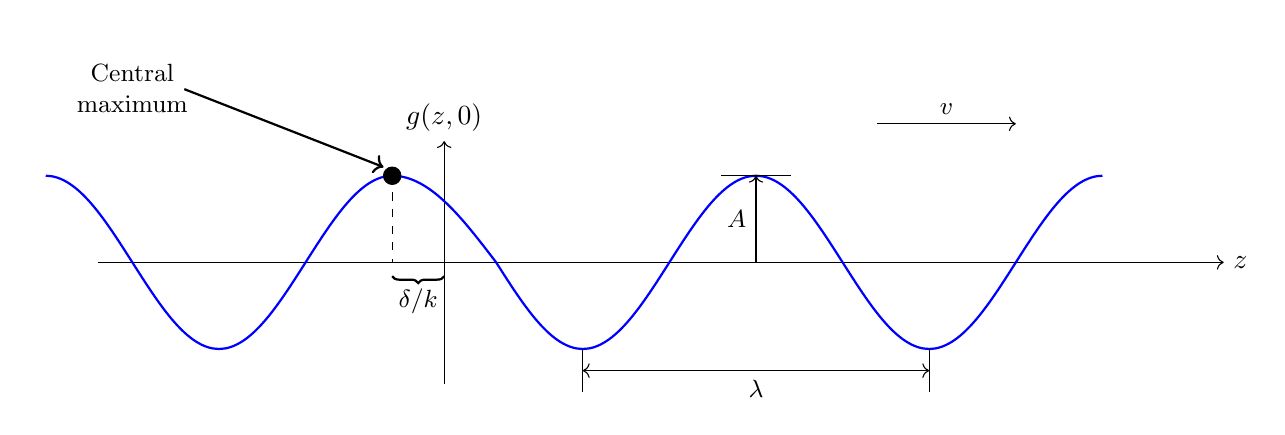
\begin{tikzpicture}[scale=1.1]
    \draw[black, ->] (-4,0) -- (9,0) node[black, anchor=west] {$z$};
    \draw[black, ->] (0,-1.4) -- (0,1.4) node[black, anchor=south] {$g(z,0)$};
    \draw[blue, thick] (-4.6,1) cos (-3.6,0);
    \draw[blue, thick] (-3.6,0) sin (-2.6,-1);
    \draw[blue, thick] (-2.6,-1) cos (-1.6,0);
    \draw[blue, thick] (-1.6,0) sin (-0.6,1);
    \draw[blue, thick] (-0.6,1) cos (0.6,0);
    \draw[blue, thick] (0.6,0) sin (1.6,-1);
    \draw[blue, thick] (1.6,-1) cos (2.6,0);
    \draw[blue, thick] (2.6,0) sin (3.6,1);
    \draw[blue, thick] (3.6,1) cos (4.6,0);
    \draw[blue, thick] (4.6,0) sin (5.6,-1);
    \draw[blue, thick] (5.6,-1) cos (6.6,0);
    \draw[blue, thick] (6.6,0) sin (7.6,1);
    %
    \draw[black, ->] (3.6,0) -- (3.6,1) node[black, left, midway] {\small $A$};
    \draw[black] (3.2,1) -- (4.0,1);
    %
    \filldraw[black] (-0.6,1) circle (0.1);
    \node[black, above] at (-3.6,1.3) {\parbox[c]{0.2\textwidth}{\begin{center} \small Central \\ maximum \end{center}}};
    \draw[black, thick, <-] (-0.7,1.1) -- (-3,2);
    %
    \draw[black, dashed] (-0.6,1) -- (-0.6,0);
	\draw[black, thick, decoration={brace, mirror, raise=5pt}, decorate] (-0.6,0) -- (0,0) node[black, midway, below=6pt] {\small $\delta/k$};
	%
	\draw[black, ->] (5,1.6) -- (6.6,1.6) node[black, midway, above] {\small $v$};
	%
	\draw[black] (1.6,-1) -- (1.6,-1.5);
	\draw[black] (5.6,-1) -- (5.6,-1.5);
	\draw[black, <->] (1.6,-1.25) -- (5.6,-1.25) node[black, midway, below] {\small $\lambda$};
\end{tikzpicture}
\caption{A sinusoidal wave train. With the passage of time, the entire wave train proceeds to the right.}
\label{fig:sinusoidalwave}
\end{figure}

At any fixed point $z$, the string vibrates up and down, undergoing one full cycle in a period
\begin{equation*}
    T = \frac{2\pi}{kv}.
\end{equation*}

\section{Electric Fields on Pointy Things}

The pointy bits on a conducting surface should produce greater electric fields then the flat bits. Let's show that numerically. Laplace's equation, in two dimensions, reads
\begin{equation}
    \nabla^2 V = \frac{\partial^2 V}{\partial x^2} + \frac{\partial^2 V}{\partial y^2} = 0.
\end{equation}

We can solve Laplace's equation numerically using a finite difference method for a rectangular region. That is, we partition a rectangle into a lattice of grid points. If the spacing in the $x$-direction is $\Delta x$, the second derivative $\frac{\partial^2 V}{\partial x^2}$ is
\begin{equation}
    \frac{\partial^2 V}{\partial x^2} = \frac{V(x + \Delta x, y) - 2V(x,y) + V(x - \Delta x, y)}{\Delta x^2}.
\end{equation}

Similarly, if the spacing in the $y$-direction is $\Delta y$, the second derivative $\frac{\partial^2 V}{\partial y^2}$ is
\begin{equation}
    \frac{\partial^2 V}{\partial y^2} = \frac{V(x, y + \Delta y) - 2V(x,y) + V(x, y - \Delta y)}{\Delta y^2}.
\end{equation}

For convenience, let's say $\Delta x = \Delta y = h$. The Laplacian operator in two-dimensions becomes
\begin{equation}
    \frac{\partial^2 V}{\partial y^2} + \frac{\partial^2 V}{\partial y^2} = \frac{V(x + h, y) + V(x - h, y) + V(x, y + h) + V(x, y - h) - 4V(x,y)}{h^2}.
\end{equation}

Then Laplace's equation becomes
\begin{gather}
    V(x + h, y) + V(x - h, y) + V(x, y + h) + V(x, y - h) - 4V(x,y) = 0 \\
    \implies \boxed{V(x,y) = \frac{V(x + h, y) + V(x - h, y) + V(x, y + h) + V(x, y - h)}{4}}.
\end{gather}

That is, the potential $V(x,y)$ is the average of its four neighboring points on the lattice. Let's make this concrete by drawing a diagram.

\begin{figure}[H]
\captionsetup{width=0.8\textwidth,labelfont={color=black,bf},textfont={color=black}}
\centering
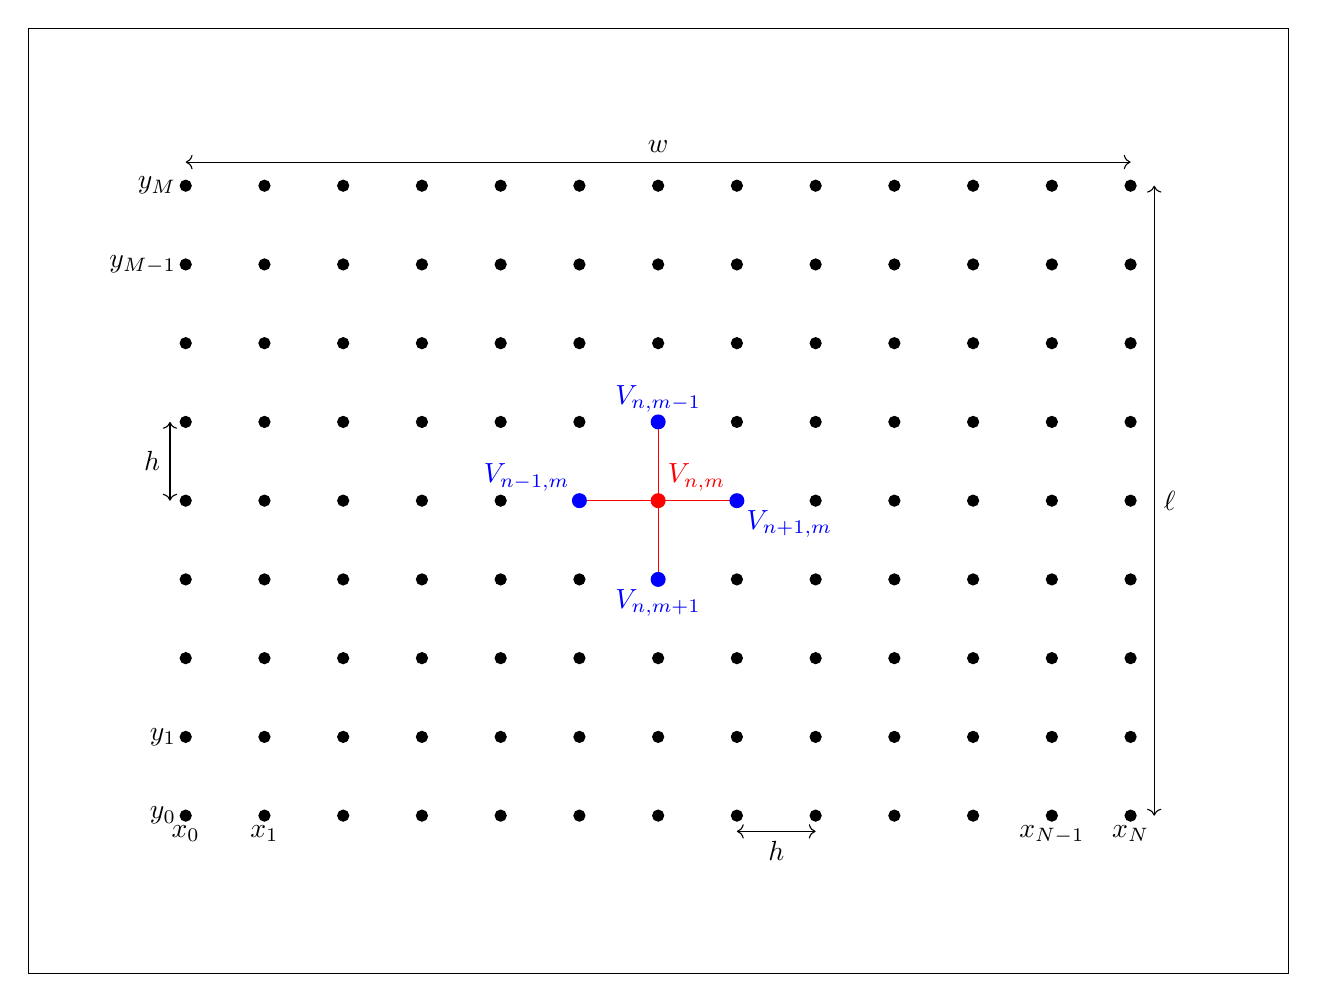
\begin{tikzpicture}[xscale=1,yscale=1]
    % Draw outside rectangle
    \draw[black] (-2,-2) rectangle (14,10);
    % Draw lattice points
    \foreach \a in {0, 1, 2, 3, 4, 5, 6, 7, 8, 9, 10, 11, 12}
    {
        \foreach \b in {0, 1, 2, 3, 4, 5, 6, 7, 8}
        {
            \filldraw[black] (\a, \b) circle (2pt);
        }
    }
    \node[black, anchor=north] at (0,0) {$x_0$};
    \node[black, anchor=north] at (1,0) {$x_1$};
    \node[black, anchor=north] at (11,0) {$x_{N - 1}$};
    \node[black, anchor=north] at (12,0) {$x_N$};
    \node[black, anchor=east] at (0,0) {$y_0$};
    \node[black, anchor=east] at (0,1) {$y_1$};
    \node[black, anchor=east] at (0,7) {$y_{M - 1}$};
    \node[black, anchor=east] at (0,8) {$y_M$};
    \draw[black, <->] (7,-0.2) -- (8,-0.2);
    \node[black, below] at (7.5,-0.2) {$h$};
    \draw[black, <->] (-0.2,4) -- (-0.2,5);
    \node[black, left] at (-0.2,4.5) {$h$};
    \filldraw[red] (6,4) circle (2.5pt) node[anchor=south west] {$V_{n,m}$};
    \draw[red] (6,3) -- (6,4) -- (6,5);
    \draw[red] (5,4)-- (6,4) -- (7,4);
    \filldraw[blue] (7,4) circle (2.5pt) node[anchor=north west] {$V_{n+1,m}$};
    \filldraw[blue] (5,4) circle (2.5pt) node[anchor=south east] {$V_{n-1,m}$};
    \filldraw[blue] (6,3) circle (2.5pt) node[anchor=north] {$V_{n,m+1}$};
    \filldraw[blue] (6,5) circle (2.5pt) node[anchor=south] {$V_{n,m-1}$};
    \draw[black, <->] (0,8.3) -- (12,8.3);
    \node[black, above] at (6,8.3) {$w$};
    \draw[black, <->] (12.3,0) -- (12.3,8);
    \node[black, right] at (12.3,4) {$\ell$};
\end{tikzpicture}
\caption{A two-dimensional lattice of points.}
\label{fig:latticegrid}
\end{figure}

As shown in Fig. (\ref{fig:latticegrid}), we partition the interval $0 < x < w$ into $N + 1$ evenly spaced points. That is,
\begin{equation}
    x_n = nh, \qquad \text{for} \quad n \in \left\{ 0, 1, \dots, N \right\}.
\end{equation}

Likewise, we divide the interval $0 < y < \ell$ into $M + 1$ evenly spaced points. That is,
\begin{equation}
    y_m = mh, \qquad \text{for} \quad m \in \left\{ 0, 1, \dots M \right\}.
\end{equation}

What follows is the implementation of this numerical method.

% If we were uploading from an external file, use the line below.
% \lstinputlisting[language=python]{corners.py}

\begin{lstlisting}[language=Python]
"""
Created on Mon Feb 03 13:12:20: 2020
Author: Nicholas D. Kostin
Description: Numerical solution to Laplace's equation for a rectangle
"""

import numpy as np, matplotlib.pyplot as plt

plt.rcParams['mathtext.fontset'] = 'stix'
plt.rcParams['font.family'] = 'STIXGeneral'

# Physical constants
eps0 = 8.85e-12 # permittivity of free space

# Dimensions of region
region_width = 120 # Horizontal length of region
region_length = 80  # Vertical length of region

# Dimensions of conucting rectangle
rectangle_width = 60  # Horizontal length of conducting rectangle
rectangle_length = 40  # Vertical length of conducting rectangle

# Location of bottom-left corner of conducting rectangle
rect_corner = 20

# Set potential at boundaries of region to be zero
boundary_potential = 0

# Dirichlet Boundary conditions on conducting rectangle
# All sides at the same potential
V_box = 9

# Set color interpolation and color map
color_interpolation = 20
color_map = plt.cm.coolwarm # dope-ass colors

# Create lattice of points
X, Y = np.meshgrid(np.arange(0, region_width), np.arange(0, region_length))

# Set array size and the interior value with some guess
V = np.ones((region_length, region_width))
V.fill(0)

# Set potential at boundaries of region
V[1, :] = boundary_potential # potential at bottom
V[region_length - 1, :] = boundary_potential # potential at top
V[:, 1] = boundary_potential # potential at left
V[:, region_width - 1] = boundary_potential # potential at right


# Set potential at boundaries of conducting rectangle
V[rect_corner, rect_corner:rect_corner + rectangle_width] = V_box # potential at bottom
V[rect_corner + rectangle_length, rect_corner:rect_corner + rectangle_width] = V_box # potential at top
V[rect_corner:rect_corner + rectangle_length, rect_corner] = V_box # potential at left
V[rect_corner:rect_corner + rectangle_length, rect_corner + rectangle_width] = V_box # potential at right

# Implement 1000 iterations (and hope that's enough for convergence)
for iteration in range(0,1000):
    for i in range(1, region_length - 1, 1):
        for j in range(1, region_width - 1, 1):
            # Conducting surfaces are equipotentials
            if rect_corner <= i <= rect_corner + rectangle_length and rect_corner <= j <= rect_corner + rectangle_width:
                V[i, j] = V[i, j]
            # Implement finite difference method                
            else:
                V[i, j] = (1/4) * (V[i - 1][j] + V[i + 1][j] + V[i][j - 1] + V[i][j + 1])

# Create array for electric field
E = np.zeros((region_length, region_width, 2))

# Compute electric field
for i in range (region_length):
    for j in range (region_width):
        # Electric field is zero inside a conductor
        if rect_corner <= i <= rect_corner + rectangle_length and rect_corner <= j <= rect_corner + rectangle_width:
            E[i, j] = [0, 0]
        # Electric field is derivative of potential otherwise
        elif i != 0 and i != region_length - 1 and j != 0 and j != region_width - 1:
            E[i, j] = [(V[i + 1, j] - V[i - 1, j])/(2), (V[i, j + 1] - V[i, j - 1])/(2)]

# Create array for magnitude of the electric field
E_magnitude = np.zeros((region_length, region_width))

# Compute the magnitude of the elctric field
for i in range (region_length):
    for j in range (region_width):
        E_magnitude[i, j] = (E[i, j, 0]**2 + E[i, j, 1]**2)**(1/2)
        
# Plot a contour map of the potential
plt.figure(1)
plt.title("Contour of Potential")
plt.contourf(X, Y, V, color_interpolation, cmap=color_map)
plt.colorbar() # Set colorbar
plt.show() # Display the color map

# Plot a contour map of the electric field magnitude
plt.figure(2)
plt.title("Contour of Magnitude of Electric Field")
plt.contourf(X, Y, E_magnitude, color_interpolation, cmap=color_map)
plt.colorbar() # Set colorbar
plt.show() # Display the color map
\end{lstlisting}

\section{Infinite Square Well Potential}

Suppose we have a quantum particle with mass $m$ in an infinite square well potential:
\begin{equation*}
    V(x) = \begin{cases} 0, & 0 \leqslant x \leqslant \infty \\ \infty & \text{otherwise} \end{cases}.
\end{equation*}

The expectation value of the position $\hat{x}$ of the particle measured in the energy eigenstate $\ket{\psi_n}$ that is represented by $\psi_n(x) = \sqrt{\frac{2}{\pi}} \sin{(nx)}$, we use
\begin{equation}
    \Braket{\psi_n | \hat{x} | \psi_n} = \int_{0}^{\pi} \psi_n^*(x)\ x\ \psi_n(x)\ dx = \frac{2}{\pi} \int_{0}^{\pi} x\ \sin^2{(nx)}\ dx = \frac{\pi}{2}.
\end{equation}

The expectation value of the momentum $\hat{p}$ in the eigenstate $\ket{\psi_n}$ is given by
\begin{equation}
    \Braket{\psi_n | \hat{p} | \psi_n} = \int_{0}^{\pi} \psi_n^*(x)\ \left( -i\hbar\frac{d}{dx} \right)\ \psi_n(x)\ dx = 0.
\end{equation}

\section{Commuting Hermitian Matrices}

Let $A, B \in \bbC^{p \times p}$ be Hermitian matrices. Prove that $AB$ is Hermitian if and only if $A$ and $B$ commute (\textit{i.e.} they don't work from home).

\begin{proof}

A matrix $\mathscr{A} \in \bbC^{p \times p}$ is Hermitian if it satisfies
\begin{equation*}
    \mathscr{A}^{\dagger} = \mathscr{A}.
\end{equation*}

That is, a matrix $\mathscr{A} \in \bbC^{p \times p}$ is Hermitian if it is its own conjugate transpose. Moreover, for $\mathscr{A} \in \bbC^{p \times q}$ and $\mathscr{B} \in \bbC^{q \times r}$, we have the identity
\begin{equation*}
    \left( \mathscr{AB} \right)^{\dagger} = \mathscr{B}^{\dagger} \mathscr{A}^{\dagger}.
\end{equation*}

We will start by proving the forward direction. That is, we will show that if $A$ and $B$ commute, then $AB$ must be Hermitian. Using the identity above to take the conjugate transpose of $AB$ we get
\begin{equation*}
    \left( AB \right)^{\dagger} = B^{\dagger} A^{\dagger}.
\end{equation*}

But since we assumed $A$ and $B$ to both be Hermitian, we have that $B^{\dagger} = B$ and $A^{\dagger} = A$. Explicitly,
\begin{equation*}
    \left( AB \right)^{\dagger} = B^{\dagger} A^{\dagger} = BA.
\end{equation*}

But since we assumed $A$ and $B$ commute, then $BA = AB$. And we have
\begin{equation*}
    \left( AB \right)^{\dagger} = B^{\dagger} A^{\dagger} = BA = AB
\end{equation*}

Thereby $AB$ satisfies the definition of a Hermitian matrix. Now we will show the reverse direction: that if $AB$ is Hermitian then $A$ and $B$ must necessarily commute. If $AB$ is Hermitian, then
\begin{equation*}
    \left( AB \right)^{\dagger} = AB
\end{equation*}

But we already showed that we can rewrite the left-hand side of the equation above as $\left( AB \right)^{\dagger} = B^{\dagger} A^{\dagger} = AB$, since we assumed $A$ and $B$ to both be Hermitian. Then we have
\begin{equation*}
    BA = AB.
\end{equation*}

And clearly, $A$ and $B$ must necessarily commute.

\end{proof}

\section{Blind Text}

\blindtext[2]

\newpage

\section{Some Results from Real Analysis}

Here we have a \emph{theorem}.

\begin{mdframed}[backgroundcolor=black!4, align=center, userdefinedwidth=40em, topline=false, bottomline = false, leftline = false, rightline = false, frametitle = {Bolzano-Weierstrass Theorem}]
Every bounded sequence has a convergent subsequence.
\end{mdframed}

What follows is a \emph{lemma}.

\begin{mdframed}[backgroundcolor=black!4, align=center, userdefinedwidth=40em, topline=false, bottomline = false, leftline = false, rightline = false, frametitle = {Lemma}]
Cauchy sequences are bounded.
\end{mdframed}

\section{Computer Colors}

HTML color codes are hexadecimal triplets representing the colors red, green and blue.

\begin{figure}[H]
\centering
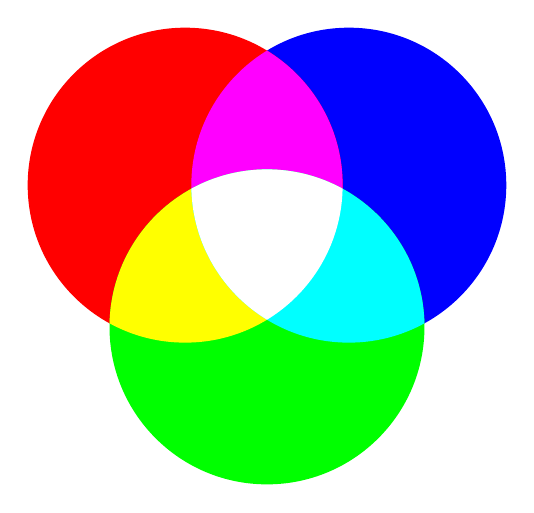
\begin{tikzpicture}[scale=0.5]
    % primary colors
    \fill[blue] (30:2.4) circle (4);
    \fill[red] (150:2.4) circle (4);
    \fill[lime] (270:2.4) circle (4);
    % secondary colors
    \begin{scope} % red + blue = purple
        \clip (150:2.4) circle (4);
        \fill[magenta] (30:2.4) circle (4);
    \end{scope}
    \begin{scope} % red + green = yellow
        \clip (270:2.4) circle (4);
        \fill[yellow] (150:2.4) circle (4);
    \end{scope}
    \begin{scope} green + blue = teal
        \clip (30:2.4) circle (4);
        \fill[cyan] (270:2.4) circle (4);
    \end{scope}
    % red + blue + green = white
    \begin{scope}
        \clip (30:2.4) circle (4);
        \clip (150:2.4) circle (4);
        \fill[white] (270:2.4) circle (4);
    \end{scope}
\end{tikzpicture}
\end{figure}

\section{Awesome Circled Numbers and Highlighting}

Here are some cool circled numbers. The first argument is whatever is to be circled, and the \colorbox{cyan}{second argument} is the background color. The \colorbox{purple}{third argument} is the outline color, and the \colorbox{red}{fourth argument} is color of the first argument.

\begin{figure}[H]
\captionsetup{width=0.8\textwidth,labelfont={color=black,bf},textfont={color=black}}
\centering
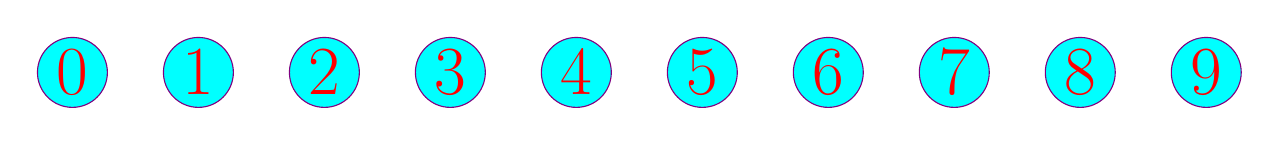
\begin{tikzpicture}[scale=1.6]
    \foreach \c in {0, 1, 2, 3, 4, 5, 6, 7, 8, 9}
    {
        \node at (\c,0) {\Huge\circled{\c}{cyan}{purple}{red}};
    }
\end{tikzpicture}
\caption*{Isn't this cool?}
\end{figure}

These circled numbers work in equations too!
\begin{equation*}
    \bigints_{\circled{$a$}{pink}{black}{black}}^{\circled{$b$}{goldenrod}{black}{black}} \Scale[2]{f(x)} \Scale[2]{dx} \hspace{1em} \Scale[2]{+} \hspace{1em} \bigints_{\circled{$b$}{goldenrod}{black}{black}}^{\circled{$a$}{pink}{black}{black}} \Scale[2]{f(x)} \Scale[2]{dx} \hspace{1em} \Scale[2]{=} \hspace{1em} \Scale[2]{\circled{0}{lime}{red}{black}}
\end{equation*}

Don't forget, however, that too much color is cringe, so be exercise caution!

\section{Consider a Graph}

Consider a graph with vertices

\begin{equation*}
    V = \left\{ 1, 2, 3, 4, 5, 6 \right\}
\end{equation*}

and edges
\begin{equation*}
    E = \left\{ 1 \to 2, 1 \to 3, 1 \to 4, 2 \to 1, 2 \to 3, 3 \to 4, 4 \to 1, 4 \to 3, 4 \to 5, 4 \to 6, 5 \to 6, 6 \to 5 \right\}
\end{equation*}

The directed graph for this vertex set $V$ and edge set $E$ is

\begin{figure}[H]
\centering
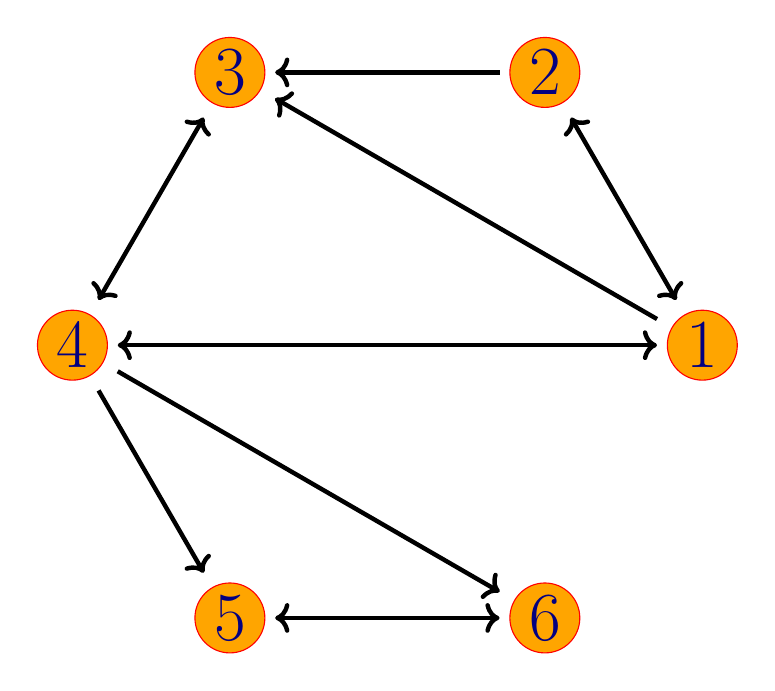
\begin{tikzpicture}
    \coordinate (vertex1) at (4,0);
    \coordinate (vertex2) at (2,3.464102);
    \coordinate (vertex3) at (-2,3.464102);
    \coordinate (vertex4) at (-4,0);
    \coordinate (vertex5) at (-2,-3.464102);
    \coordinate (vertex6) at (2,-3.464102);
    %
    \node at (vertex1) (nodeV1) {\Huge\circled{1}{orange}{red}{nkostincolor}};
    \node at (vertex2) (nodeV2) {\Huge\circled{2}{orange}{red}{nkostincolor}};
    \node at (vertex3) (nodeV3) {\Huge\circled{3}{orange}{red}{nkostincolor}};
    \node at (vertex4) (nodeV4) {\Huge\circled{4}{orange}{red}{nkostincolor}};
    \node at (vertex5) (nodeV5) {\Huge\circled{5}{orange}{red}{nkostincolor}};
    \node at (vertex6) (nodeV6) {\Huge\circled{6}{orange}{red}{nkostincolor}};
    %
    \draw[black, ultra thick, <->] (nodeV1) -- (nodeV2);
    \draw[black, ultra thick, ->] (nodeV2) -- (nodeV3);
    \draw[black, ultra thick, <->] (nodeV3) -- (nodeV4);
    \draw[black, ultra thick, ->] (nodeV4) -- (nodeV5);
    \draw[black, ultra thick, <->] (nodeV5) -- (nodeV6);
    \draw[black, ultra thick, <->] (nodeV1) -- (nodeV4);
    \draw[black, ultra thick, ->] (nodeV1) -- (nodeV3);
    \draw[black, ultra thick, ->] (nodeV4) -- (nodeV6);
\end{tikzpicture}
\end{figure}

\section{A Particle in 3D}

A particle in 3D has mass $m$ and is in the potential $V(x,y,z) = \frac{1}{2} m \omega^2 \left( x^2 + y^2 + z^2 \right).$

\subsection{Energies of the Lowest Four Eigenstates}

Suppose we need to find the energies of the four lowest eigenstates of the Hamiltonian and their corresponding degeneracies. We can start by expanding the potential as
\begin{equation*}
    V(x, y, z) = \underbrace{\frac{1}{2} m \omega^2 x^2}_{V_x(x)} + \underbrace{\frac{1}{2} m \omega^2 y^2}_{V_y(y)} + \underbrace{\frac{1}{2} m \omega^2 z^2}_{V_z(z)}.
\end{equation*}

And the total eigenenergy is
\begin{equation}
    E_{n_x n_y n_z} = E_{n_x} + E_{n_y} + E_{n_z} = \hbar \omega \left( n_x + \frac{1}{2} \right) + \hbar \omega \left( n_y + \frac{1}{2} \right) + \hbar \omega \left( n_z + \frac{1}{2} \right) \label{eqn:3dQHO:eigenenergy}
\end{equation}

where $n_x, n_y, n_z = 0, 1, 2, \dots$ are independent from each other. The ground state should have $n_x = n_y = n_z = 0$, so its energy is given by

\begin{equation*}
    E_{000} = 3 \hbar \omega \left( \frac{1}{2} \right) = \frac{3}{2} \hbar \omega.
\end{equation*}

The first excited state has energy
\begin{equation*}
    \underbrace{E_{100} = E_{010} = E_{001}}_{\text{degeneracy 3}} = \frac{\hbar}{\omega} \left( \frac{3}{2} + \frac{1}{2} + \frac{1}{2} \right) = \frac{5}{2} \hbar \omega.
\end{equation*}

The second excited state has energy
\begin{equation*}
    \underbrace{E_{200} = E_{020} = E_{002} = E_{110} = E_{101} = E_{011}}_{\text{degeneracy 6}} = \frac{\hbar}{\omega} \left( \frac{5}{2} + \frac{1}{2} + \frac{1}{2} \right) = \frac{7}{2} \hbar \omega.
\end{equation*}

And finally, the third excited state has energy
\begin{equation*}
    \underbrace{\left\{ \begin{array}{l} E_{300} = E_{030} = E_{003} = E_{111} = E_{102} \\[0.4em] E_{120} = E_{201} = E_{021} = E_{210} = E_{012} \end{array} \right\}}_{\text{degeneracy 10}} = \frac{\hbar}{\omega} \left( \frac{7}{2} + \frac{1}{2} + \frac{1}{2} \right) = \frac{9}{2} \hbar \omega.
\end{equation*}

These results are summarized in the table below.

\begin{table}[H]
\centering
\captionsetup{width=0.8\textwidth,labelfont={color=black,bf},textfont={color=black}}
\caption{Energies and corresponding degeneracies of the 3D QHO}
\begin{tabular}{@{}ccc@{}}
\toprule
State & Energy & Degeneracy \\ \midrule
\multicolumn{1}{c|}{Ground state} & \multicolumn{1}{c|}{$\displaystyle \frac{3}{2}\hbar\omega$} & 1 \\[1em]
\multicolumn{1}{c|}{First excited state} & \multicolumn{1}{c|}{$\displaystyle \frac{5}{2}\hbar\omega$} & 3 \\[1em]
\multicolumn{1}{c|}{Second excited state} & \multicolumn{1}{c|}{$\displaystyle \frac{7}{2}\hbar\omega$} & 6 \\[1em]
\multicolumn{1}{c|}{Third excited state} & \multicolumn{1}{c|}{$\displaystyle \frac{9}{2}\hbar\omega$} & 10 \\ \bottomrule
\end{tabular}
\end{table}

\subsection{Degeneracy of an Arbitrary Excited State}

Now suppose we need to find the degeneracy $g_n$ of the $n^{th}$ excited state as a function of $n$. For our three-dimensional harmonic oscillator, we can define
\begin{equation*}
    n = n_x + n_y + n_z.
\end{equation*}

It follows from Eq. (\ref{eqn:3dQHO:eigenenergy}) that the energy is strictly a function of $n$. That is, any combination of $n_x$, $n_y$, and $n_z$, as long as they produce the same $n$, will yield the same energy. Such states are said to be \emph{degenerate}. Our goal is to find how many possible combinations of $n_x$, $n_y$, and $n_z$ exist for a given $n$.

To explicitly determine the degeneracy $g_n$ for a given state, we fix the value of $n$. Because of the restriction imposed by setting $n = n_x + n_y + n_z$, we really have two free parameters (say, $n_x$ and $n_y$). We let $n_x$ assume any allowable integer value:
\begin{equation*}
    n_x \in \left\{ 0, 1, \dots, n \right\}.
\end{equation*}

Then $n_y$ can assume any integer value given the sum $n_x + n_y$ does not exceed $n$:
\begin{equation*}
    n_y \in \left\{ 0, 1, \dots, n - n_x \right\}.
\end{equation*}

In particular, for any value of $n_x$, there are $n - n_x + 1$ unique choices for $n_y$ (note the size of the set of permissible $n_y$ values). Finally, $n_z$ is automatically fixed:
\begin{equation*}
    n_z = n - n_x - n_y.
\end{equation*}

For each permissible value of $n_x$ (from $0$ to $n$), there are $n - n_x + 1$ choices for $n_y$. Summing the number of these choices for all allowable values of $n_x$ yields
\begin{align*}
    \sum\limits_{n_x = 0}^n \left( n - n_x + 1 \right) &= \left(n + 1\right) + n + \left(n - 2\right) + \cdots + \cancelto{0}{\left(n - n\right)} \\
                                                       &= \frac{\left(n+1\right) \left(n+2\right)}{2}.
\end{align*}

The series above is well known. Thus, we find that the degeneracy is
\begin{equation*}
    g_n = \frac{\left(n+1\right) \left(n+2\right)}{2}.
\end{equation*}

\end{document}
